% -- Encoding UTF-8 without BOM
% -- XeLaTeX => PDF (BIBER)

\documentclass[]{cv-style}          % Add 'print' as an option into the square bracket to remove colours from this template for printing. 
                                    % Add 'espanol' as an option into the square bracket to change the date format of the Last Updated Text

\sethyphenation[variant=british]{english}{} % Add words between the {} to avoid them to be cut 

\begin{document}

\header{Joslenne}{Pe$\tilde{n}$a}           % Your name
\lastupdated

%----------------------------------------------------------------------------------------
%	SIDEBAR SECTION  -- In the aside, each new line forces a line breakhttps://www.overleaf.com/project/5c364006010617222f58aa77
%----------------------------------------------------------------------------------------
\begin{aside}
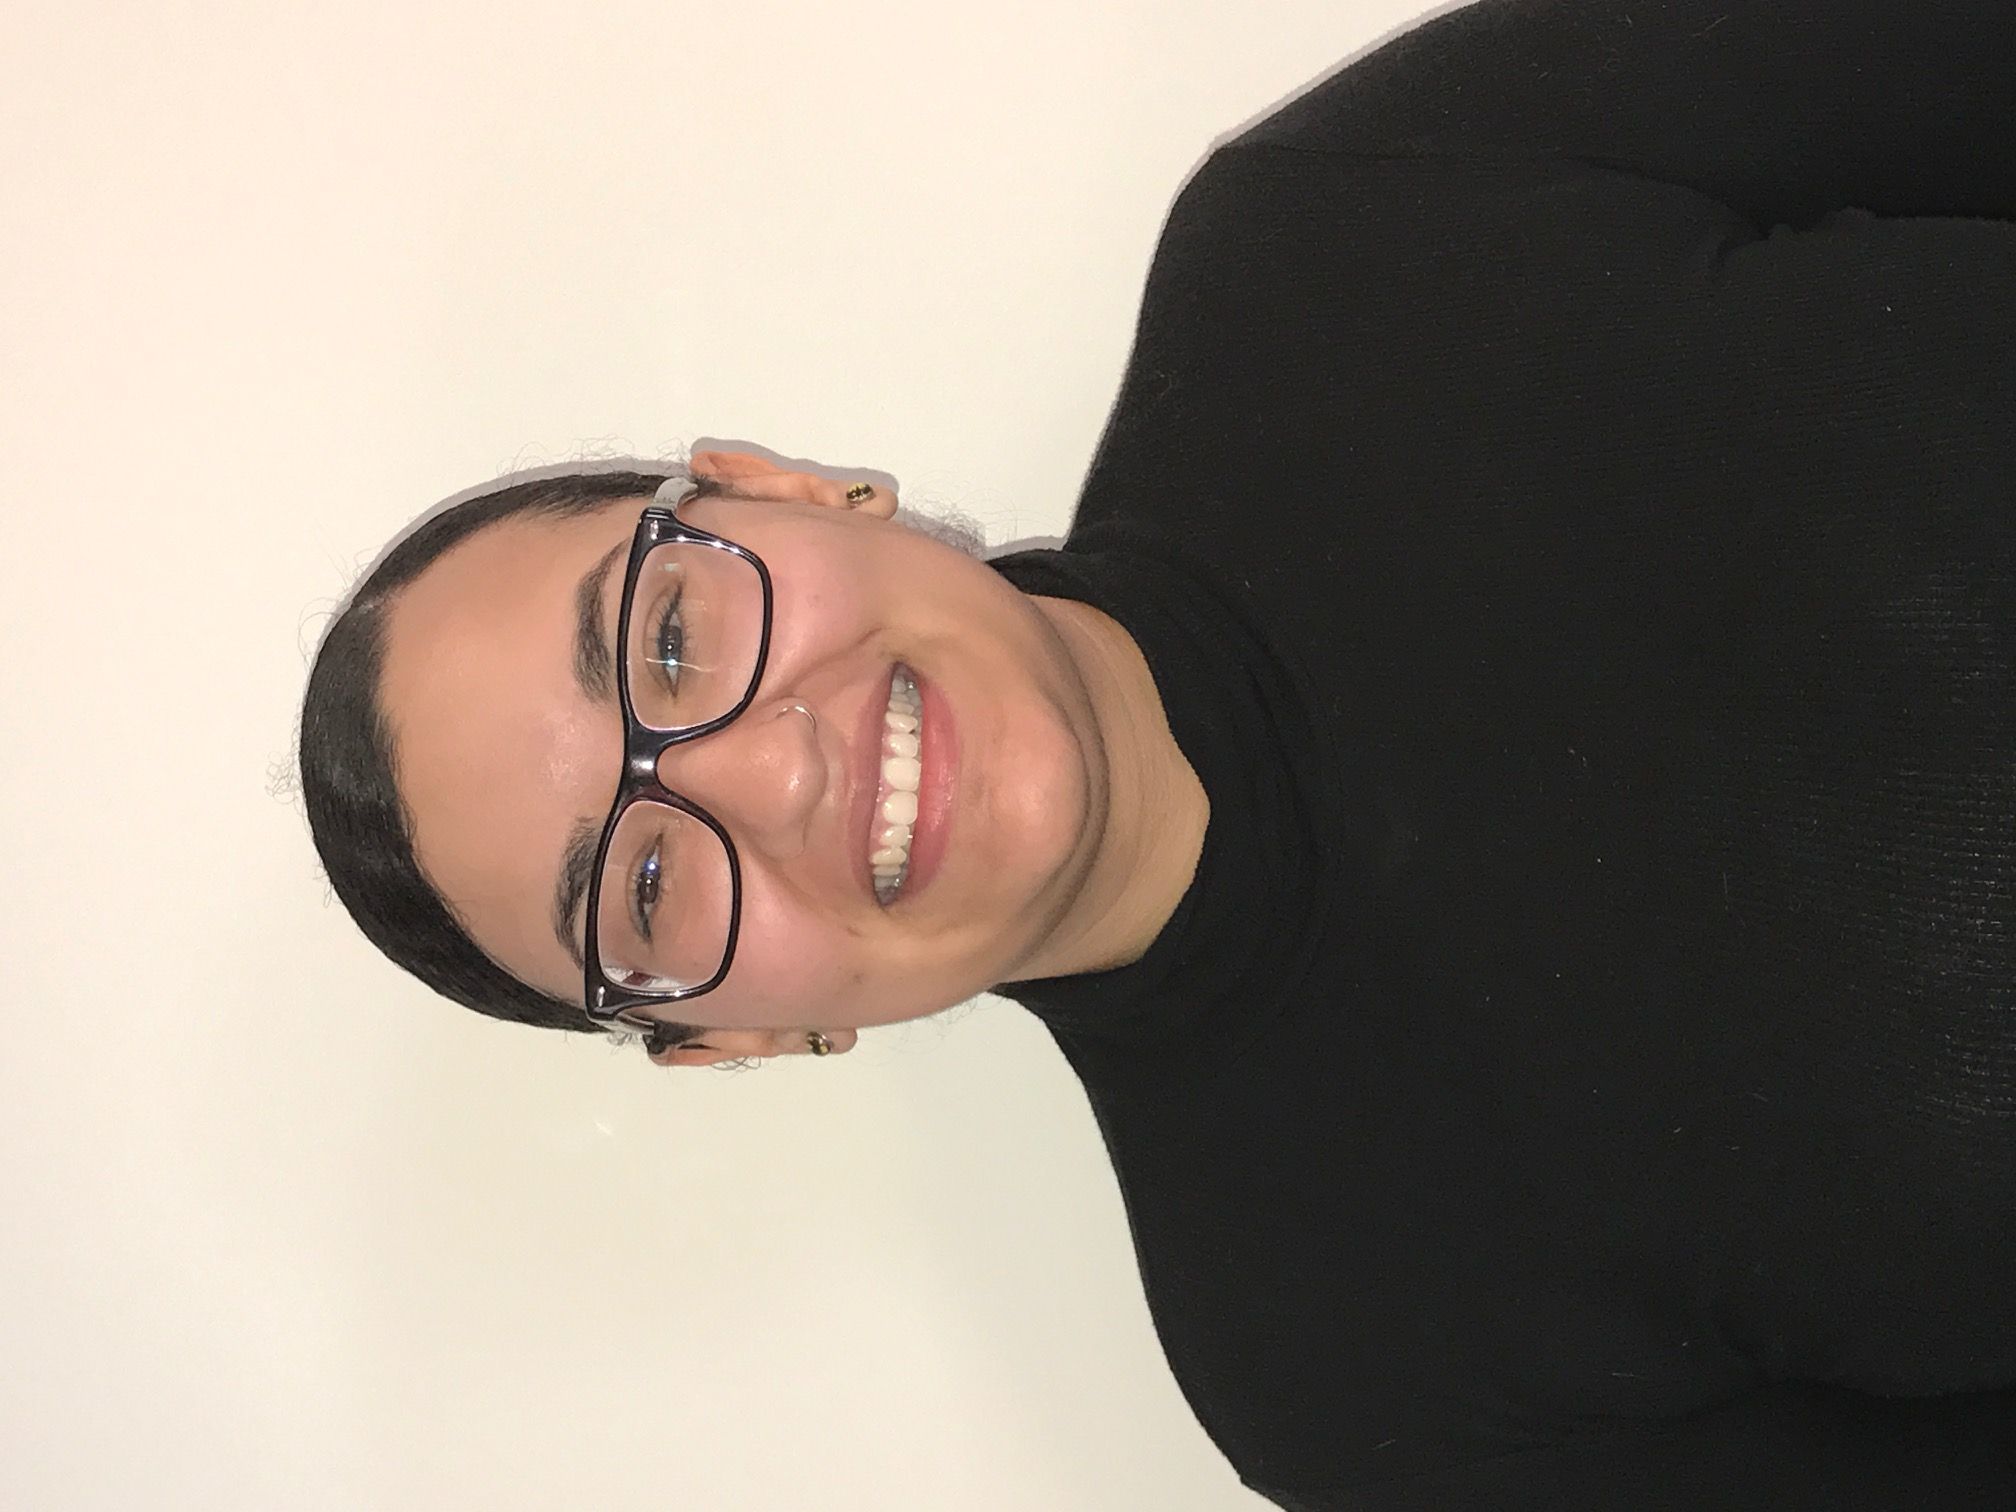
\includegraphics[width=\linewidth, angle=270]{IMG_2797}
%
\textbf{*Willing to Relocate}
\section{contact}
E311 Westgate Building
University Park, PA 16802
United States
~
917.596.6547
~
jop5190@psu.edu
%
\section{links}
%sites.psu.edu/joslennepena
linkedin.com/in/jossp
twitter.com/jpena831
%
\end{aside}


%----------------------------------------------------------------------------------------
%	EDUCATION SECTION
%----------------------------------------------------------------------------------------
\section{education}
\vspace{-0.3cm}
\begin{entrylist}
%------------------------------------------------
\entry
{2015--now}
{Ph.D. Candidate {\normalfont in Informatics}}
{The Pennsylvania State University}
{\jobtitle{Advisor: Mary Beth Rosson \newline
Specialization: Human-Computer Interaction \newline
Dissertation Title: Promoting Computational Grounding through Informal Coding Workshops for Non-Programmers}}
\textbf{Anticipated End Date: July 2020}
%{\vspace{-0.01cm}} 
%------------------------------------------------
\entry 
{2013--2015}
{M.S. {\normalfont in Information Sciences and Technology}}
{The Pennsylvania State University}
{{\normalfont Conferred August 2015}}
%{\vspace{-0.3cm}}
%------------------------------------------------
\entry
{2009--2013}
{B.A. {\normalfont in Multimedia Web Design and Development}}
{University of Hartford}
{{\normalfont Conferred May 2013 \newline {\jobtitle{Cum Laude, President's List}}}}
%------------------------------------------------
\end{entrylist}
%----------------------------------------------------------------------------------------
%	SKILLS SECTION
%----------------------------------------------------------------------------------------
\section{skills}
  \vspace{-0.2cm}
  
{\textbf{Tools} | HTML, CSS, JavaScript/JQuery, Bootstrap, Wordpress, Joomla, Drupal, Scratch, Photoshop, Jing, Blackboard LMS, Canvas LMS, Axure RP, Audacity, Balsamiq, SPSS, Python/Django, Invision, Excel, Word, Visio, Powerpoint, Qualtrics, Morae, \LaTeX{}, Tableau, D3.js}

{\textbf{Research} | Interviews, Surveys, Focus Groups, Prototyping, Usability Heuristics, Think Alouds, Scenarios, Personas, Eye Tracking, Task Analysis, Metric Development, Affinity Diagramming, Electromyopgraphy (EMG) procedures, BioSemi ActiveTwo Equipment}

\iffalse
%----------------------------------------------------------------------------------------
%	CURENNT APPOINTMENTS SECTION
%----------------------------------------------------------------------------------------
\section{current appointments}
\vspace{-0.2cm}
\begin{entrylist}
%------------------------------------------------
\entry
  {2020-Now}
  {Adjunct Professor, Graphic and Web Design}
  {}
  {\jobtitle{Minneapolis College of Art and Design, Minneapolis, MN}\\
  I am designated within the Continuing Education program to teach online courses for students toward their M.A. in Graphic and Web Design program. }
%------------------------------------------------
\entry
  {2018-Now}
  {Graduate Research Assistant - Coding Workshop Consultant}
  {}
  {\jobtitle{Schreyer Business Library, Penn State, University Park, PA}\\
 Leading the implementation of a web development coding workshop targeted to female and gender diverse Penn State students, faculty, and staff at University Park. Responsible for creating workshop curriculum, teaching, recruitment and selection of workshop participants, facilitating workshop content, delivery of content, and assessment of workshop for research purposes, presentation and publication. I am also leading research efforts on investigating the impacts of the workshop on participants. Responsible for the direction of an undergraduate intern: \textbf{Katie O'Leary} and facilitator: \textbf{Sara Krum} }
%------------------------------------------------
\end{entrylist}

\fi



%----------------------------------------------------------------------------------------
%	RESEARCH EXPERIENCE SECTION
%----------------------------------------------------------------------------------------
\section{research experience}
\vspace{-0.2cm}
\begin{entrylist}
%------------------------------------------------
\entry
  {2018-Now}
  {Graduate Research Assistant - Coding Workshop Consultant}
  {}
  {\jobtitle{Schreyer Business Library, Penn State, University Park, PA}\\
  Leading the implementation of a web development coding workshop targeted to female and gender diverse Penn State students, faculty, and staff at University Park. Responsible for creating workshop curriculum, teaching, recruitment and selection of workshop participants, facilitating workshop content, delivery of content, and assessment of workshop for research purposes, presentation and publication. I am also leading research efforts on investigating the impacts of the workshop on participants. Responsible for the direction of an undergraduate intern: \textbf{Katie O'Leary} and facilitator: \textbf{Sara Krum} }
%------------------------------------------------
\entry
  {2017--2018}
  {Research Associate, (14 month internship)}
  {}
  {\jobtitle{Human-Centered Systems (HCS), Honeywell Aerospace, Golden Valley, MN \newline Manager: Olu Olofinboba}\\ 
  Specifically housed in the crew interface and platform systems (CIPS) group. Performing all aspects of human-centered design from concept development efforts, conducting research studies, to conducting and reporting research analyses in various projects. Selected projects are described below.

 \begin{itemize}
  \item[]
  	{\textbf{Program: Strengthening Human Adaptive Reasoning and Problem-Solving (SHARP)}}
	{\jobtitle{Project Manager: Santosh Mathan \newline Supervisor: Michael Dillard}}\\
IARPA-funded program developing a cutting-edge regimen of game-based cognitive training and brain stimulation, designed to improve fluid intelligence. Worked in collaboration with Oxford University, Harvard University, Northeastern University and Simcoach Entertainment to develop a game-based training grounded in psychological theory, which targets unique combinations of component processes of fluid intelligence (Robot Factory). The task set served as the foundation of the adaptive training game, which has since been nominated for several awards at the Serious Games Showcase \& Challenge. Participated in data collection efforts with the MITRE corporation serving as a test administrator which involved directly interfacing with participants such as consenting, recruiting, and screening as well as administering their test sessions.
  \item[]
  	{\textbf{Program: NextGen Flight Deck Multifunction Touch Screen Controls: Research on Human Factors Considerations and Development of Recommendations for Enhancements to FAA Guidance Material}}\\
  {\jobtitle{Project Manager: Sonia Dodd \newline Collaborator: Jeff Lancaster}}\\
FAA-funded program concerned with producing information that will inform Aircraft Certification personnel who will evaluate the use of multi-touch screen controls on the flight deck. Using a human factors approach that encompasses identifying stakeholder issues with interface, iterative design and prototyping, and eliciting feedback through objective and subjective performance measures. Directly involved with experimental design, artifact designs, literature reviews, administering EMG equipment and running pilot experiments using a motion simulator.
\item[]
     {\textbf{Program: Intelligent Flight Deck}}\\
  {\jobtitle{Project Manager: Barbara Holder \newline
  Supervisor: Chaya Garg}}\\
Using a human factors approach that encompasses identifying stakeholder issues with intelligent flight decks and specifically single pilot operations. This program aims to develop variable automated operations to enhance the aircraft. Validate software integration to existing platforms and demonstrate intelligent human-automation interaction interfaces and finally create a framework for collaborative human-autonomy teams. My tasks involve literature searches to determine state-of-the-art approaches in intelligent flight decks that use machine learning algorithms and artificial intelligence with the goal for conceptualizing designs. Other tasks include paper write-ups for customers and stakeholders, brainstorming and design sessions for concepts, and presentation updates. 
\iffalse BELOW ARE COMMENTS
	\item[]
     {\textbf{Program: Distributed Data Analytics}}\\
  {\jobtitle{Project Manager: Emmanuel Letsu-Dake}}\\
This program is concerned with the use of big data analytics to monetize the digital exhaust generated by avionics products to optimize and provide valuable insight to Honeywell stakeholders. The idea of the connected aircraft, data-centric aircraft, and distributed analytics on the flight deck seek to enhance the aerospace industry. My tasks involve creating use cases, prototyping, and visualization development for the purposes of meaningfully displaying pilot performance through discrete events.\\
\item[]
     {\textbf{Program: Intelligent Flight Deck}}\\
  {\jobtitle{Project Manager: Barbara Holder \newline
  Supervisor: Chaya Garg}}\\
Using a human factors approach that encompasses identifying stakeholder issues with intelligent flight decks and specifically single pilot operations. This program aims to develop variable automated operations to enhance the aircraft. Validate software integration to existing platforms and demonstrate intelligent human-automation interaction interfaces and finally create a framework for collaborative human-autonomy teams. My tasks involve literature searches to determine state-of-the-art approaches in intelligent flight decks that use machine learning algorithms and artificial intelligence with the goal for conceptualizing designs. Other tasks include paper write-ups for customers and stakeholders. \\

\item[]
     {\textbf{Program: Virtual Reality Control Station}}\\
  {\jobtitle{Project Manager: Erin Alves}}\\
This program aims to explore the use of UAVs in industrial settings. Using a human factors approach, field observations are being done in various site locations to better understand how everyday engineers may use UAVs to help their efforts. Experiments and evaluations will be run to determine the differences between use and procedure. Last but not least, recommendations will be made for future design, operation protocol, and to provide a usable solution for the customer. \\
\fi
\end{itemize}}
%------------------------------------------------
\end{entrylist}

\begin{entrylist}
%------------------------------------------------
\entry
  {2016--2018}
  {Graduate Research Assistant, Exploring Heuristics and Designing Interface Cues for Secure and Trustworthy Computing}
  {}
  {\jobtitle{Center for Human-Computer Interaction, Penn State, University Park, PA}\\
  In an NSF-funded program, I conducted user studies on semi-functional interfaces designed by Axure; our team was interested in how the design of these interfaces have an effect on online information disclosure as well as privacy. Personally tasked with recruitment, data collection, consenting, data analysis, and publication writing.}
%------------------------------------------------
\entry
  {2016--Now}
  {Graduate Research Assistant, Minimalist Learning with Tableau}
  {}
  {\jobtitle{Computer-Supported Collaboration and Learning Lab, Penn State, University Park, PA}\\
  Began a project and led an undergraduate researcher in devising a user study that will elicit design features through task-based prompts and minimalist instructional guides; will conduct interviews and rapid prototyping to refine Tableau. Conducted concept development efforts, submitted an IRB protocol form, and aggregated appropriate literature.}
%------------------------------------------------
\entry
  {2014--2016}
  {Graduate Research Assistant, Evaluation of a Technology Education Pipeline Project}
  {}
  {\jobtitle{Computer-Supported Collaboration and Learning Lab, Penn State, University Park, PA}\\
  With other collaborators designed and developed iTech Academy, an online community, using Drupal and investigated its role in enhancing K-12 interest in computing careers in two contexts (summer camps and workshops). Led undergraduate researchers in recruiting, data collection efforts, system development, and publication writing. Undergraduate researchers working with us: \textbf{Dana Cinque, Ana Segura, Sarah-Alice Hanna, Adrian Negron, Jin Zhang}}
%------------------------------------------------
\entry
  {2014--2015}
  {Dialectal Learning with Piazza}
  {}
  {\jobtitle{Computer-Supported Collaboration and Learning Lab, Penn State, University Park, PA}\\
 Our lab group re-purposed the use of Piazza, a QandA system, into a discussion based tool. Through several implementations in various classes and asking students to interface with the tool, we investigated the effectiveness of Piazza in argumentation building and critical thinking, as well as eliciting design requirements to potentially improve this system. Contributed through concept development efforts and lab discussions.}
%------------------------------------------------
\entry
  {2013--2015}
  {An Investigation of Design Features for Inverted Classroom Support Technology}
  {}
  {\jobtitle{Computer-Supported Collaboration and Learning Lab, Penn State, University Park, PA}\\
  This work culminated as a result of a course project with Dr. Eileen Trauth and developed into my Master's Thesis research. I was concerned with how university instructors involved in STEM domains are appropriating unconventional teaching methods and the technologies they use to address their needs. Interviewed instructors across campus to investigate their current technical practices in instruction as well as their 'flipping' teaching approach; used interviews to elicit design features for design prototypes}
%------------------------------------------------
 \entry
  {2012}
  {Developer, Requirements Gatherer, Usability Tester, and Technical Writer}
  {}
  {\jobtitle{Mathematics Department, University of Hartford, West Hartford, CT}\\
   For my senior capstone project, I took on various roles in the development of a web application using Joomla CMS that tested a new pedagogical method (flipped classroom) for teaching calculus. I worked closely with a team of students in the design, development, and implementation of the project through an agile methodology process. In the different stages, I aided in creating interview scripts, running participants in a usability test, and writing documentation.}
%------------------------------------------------ 
\entry
  {2011--2013}
  {Computer Application Support Specialist}
  {}
  {\jobtitle{Faculty Center for Learning Development, University of Hartford, West Hartford, CT}\\
  Assisted faculty with software and hardware issues through the phone and walk-in appointments; wrote technical documentation and tutorials for educational technologies; maintained CMS-based website; provided support for Blackboard LMS such as troubleshooting modules and course tasks.} 
%------------------------------------------------
\end{entrylist}

%----------------------------------------------------------------------------------------
%	TEACHING EXPERIENCE SECTION
%----------------------------------------------------------------------------------------
\section{teaching experience}
\begin{entrylist}
%------------------------------------------------
\entry
{Summer 2019}
  {i3 PhD Teaching Fellow}
  {}
  {\jobtitle{i3 institute in the School of Information at the University of Pittsburgh \newline 
  Programming Module - 25 students}\\ 
  This module was co-taught with another Teaching Fellow \textbf{(Aisling Quigley)} and the goal was to expose students to various tools in the research process for data collection and ethics, data analysis, and visualization. Specifically, the module focused on teaching students how to scrape twitter data using python and visualizing data. Students were to leave with an understanding of what tools and resources to aid in research especially the considerations made in tool selection per task.  }
%------------------------------------------------
\entry
{Spring 2019}
  {Guest Lecturer}
  {}
  {\jobtitle{College of Information Sciences and Technology at Penn State \newline 
  IST331 – Organization and Design of Information Systems - Resident Course}\\ 
  This human-computer interaction (HCI) course focused on concepts of design and human factors through the lens of usabilty and user experience. I was invited by Dr. Patrick Dudas to teach one class session on errors in HCI.}
%------------------------------------------------
\entry
{July 2017}
{Graduate Online Teaching Certificate \newline
OL 2050: Essentials of Online Teaching for Graduate Students}
{}
{
Earned certificate in online teaching in higher education.
Learned about creating, and managing a learning environment,
engaging learners, assessing and evaluating learners, and further
developing professional learning and ethical practices}
%------------------------------------------------
\entry
  {Spring 2017}
  {Graduate Teaching Assistant}
  {}
  {\jobtitle{College of Information Sciences and Technology at Penn State \newline 
  IST331 – Organization and Design of Information Systems – 48 students – Resident Course}\\ 
  This human-computer interaction (HCI) course focused on concepts of design, practical methods, and ideas associated with visualization based on Don Norman's ideologies. I assisted Dr. Patrick Dudas with grading, course preparation, and delivery of course materials. I developed grading rubrics, created new course content, and worked closely with students on their final projects. We also implemented the Canvas LMS during the course of the semester. Lectured on special topics such as crowdsourcing methods and human errors in design.
  }
%------------------------------------------------
\entry
  {Spring 2017}
  {Graduate Teaching Assistant}
  {}
  {\jobtitle{College of Information Sciences and Technology at Penn State \newline 
  IST331 – Organization and Design of Information Systems – 54 students – Resident Course}\\ 
  This human-computer interaction (HCI) course focused on concepts of design and human factors through the lens of cognitive science. I assisted Dr. Mike McNeese with grading, course preparation, and delivery of course materials. I developed grading rubrics, created new course content, and worked closely with students on their final projects. Handled correspondences with students as well as held one-on-one appointments as needed. Led an undergraduate learning assistant and also implemented the Canvas LMS during the course of the semester. Single-handedly graded all student assignments except final course papers and lectured on special topics such as crowdsourcing methods and human errors in design.
  }
%------------------------------------------------
\entry
  {Fall 2016}
  {Graduate Teaching Assistant}
  {}
  {\jobtitle{College of Information Sciences and Technology at Penn State \newline 
  IST440W – Information Sciences and Technology Integration and Problem Solving - 50 students - Resident Course}\\ 
  This capstone course focuses on group work and the duration of the software development life cycle and is required for undergraduate senors. Student groups manage a project for a real-world client following a problem-based and writing intensive approach. Students reported weekly progress in presentation format and moved through different phases of the life cycle within the semester. I assisted Dr. Mike Hills with grading, course preparation, and delivery of course materials. I developed grading rubrics, created new course content, and worked closely with students on their final projects. 
  }
%------------------------------------------------
\entry
  {Summer 2016}
  {Instructor}
  {}
  {\jobtitle{iTech Academy Summer Camp – College of IST at Penn State}\\ 
  I designed and developed two week long camp curricula that included lesson presentations, handout tutorials, and videos. I led instruction with hands-on activities and the introduction of basic concepts in topics related to JavaScript, HTML, CSS and Scratch. Both camp courses averaged 30 high schoolers/middle schoolers per camp. 
  }
%------------------------------------------------
\entry
  {Spring 2016}
  {Graduate Teaching Assistant}
  {}
  {\jobtitle{College of Information Sciences and Technology at Penn State \newline 
  IST331 – Organization and Design of Information Systems – 48 students – Resident Course}\\ 
  This human-computer interaction (HCI) course focused on theoretical concepts of design. I assisted Dr. Tamara Peyton with grading, course preparation, and delivery of course materials. I developed grading rubrics, created new course content, and worked closely with students on their final projects. We also implemented the Canvas LMS during the course of the semester.  
  }
%------------------------------------------------
\end{entrylist}  

\begin{entrylist}
%------------------------------------------------
\entry
  {Fall 2015}
  {Graduate Teaching Assistant}
  {}
  {\jobtitle{College of Information Sciences and Technology at Penn State \newline 
  IST110 – Information, People and Technology – 55 students – World Campus Course}\\ 
  This is a freshman introductory course held online. I assisted Gary Heberling with grading, course preparation, and delivery of course materials. I assist students online through forum discussions and virtual office hours. I also recorded weekly online sessions using Blackboard Collaborate with Professor Heberling to provide students a virtual presence. 
  }
%------------------------------------------------
\entry
  {Fall 2014}
  {Graduate Teaching Assistant}
  {}
  {\jobtitle{College of Information Sciences and Technology at Penn State \newline 
  IST413 – Usability Engineering – 40 students – Resident Course }\\ 
  I assisted Dr. Patrick Shih with grading, course preparation, and delivery of course materials. I developed grading rubrics, created new course content, and worked closely with students on their final projects. External products were used such as Pebble Watch and FitBit for development purposes. This course is a follow-up to IST 331 here we focus on methods and application of concepts learned in the previous HCI course. 
  }
%------------------------------------------------
\entry
  {2014}
  {Teaching Assistant}
  {}
  {\jobtitle{iTech Academy Summer Camp – College of IST at Penn State}\\ 
  I assisted the lead instructor with demos of hands-on activities and the introduction of basic concepts in topics related to web design, programming, robotics, cyber security, and animation. I also provided guidance and feedback to the students. I aided four different week-long intensive camp courses averaging 30 high schoolers/middle schoolers per camp. 
  }
%------------------------------------------------ 
\entry
  {2011, 2012}
  {Instructor}
  {}
  {\jobtitle{Columbia University, iD Tech Camps}\\
  I taught children from the ages of 7-13 fundamental programming and game design concepts using Scratch, Photoshop, and Multimedia Fusion 2 Developer. I created lesson plans, administered review sessions, and assisted in their development of a week-long final project and participated in various meetings with parents. Further, I planned physical activities as well as challenging mental activities. There were 8 children per weekly camp course for the duration of each summer.}
%------------------------------------------------
\end{entrylist}
  
%----------------------------------------------------------------------------------------
%	PUBLICATIONS SECTION
%----------------------------------------------------------------------------------------

\section{publications and presentations}
  \vspace{-0.2cm}

\subsection{refereed/lightly-refereed conference papers and posters}
{\textbf{[P.11] Peña, J.} (2019, October). Design, Implementation, and Reflections on the Teaching of Computer Programming Modules to Underrepresented Students. To Appear In SITE - Society for Information Technology \& Teacher Education 2020}

{\textbf{[P.11]} Salac, J., {\textbf{Peña, J.}}, and Lytle, N. (2020, March). You Are Not Alone: Building Community Among Graduate Students in CS Education Research.In Proceedings of Special Interest Group on Computer Science Education (SIGCSE 2020). ACM, New York, NY, USA}

{\textbf{[P.10] Peña, J.}, \& Rosson, M.B. (2019, October). Reaching Out to Diverse Learners with Non-Formal Workshops on Computing Concepts and Skills. To Appear In Proceedings of the IEEE Symposium on Visual Languages and Human-Centric Computing (VL/HCC)}

{\textbf{[P.9] Peña, J.}. (2019, July). Seeding the Computational Skills of Diverse Non-programmers through Non-formal Workshops. In Proceedings of the 2019 ACM Conference on International Computing Education Research (pp. 347-348). ACM.}

{\textbf{[P.8] Peña, J.}, Cole, Carmen, \& Rosson, M.B. (2019, February). Code For Her: Exploring Female and Gender-Diverse Computing Workshops for Faculty, Staff, and Students. In Proceedings of the 50th ACM Technical Symposium on Computer Science Education. ACM.{\jobtitle{\textasciitilde 29\% acceptance rate}}}

{\textbf{[P.7] Peña, J.}, \& Rosson, M.B., Ge, J., Jeong, E., Sundar, S.S., Kim, J., Gambino, A. (2018, March). An Exploration of Design Cues for Heuristic-Based Decision-Making about Information Sharing. In International Conference on Information (pp. 677-683). Springer, Cham.{\jobtitle{\textasciitilde 30\% acceptance rate}} 

{\textbf{[P.6] Peña, J.}, (2017, December). Leveraging personal experience for academic research and outreach. XRDS 24, 2 (December 2017), 34-37. DOI: https://doi.org/10.1145/3155122 }}

{\textbf{[P.5] Peña, J.}, Aritajati, C., \& Rosson, M.B. (2016). The role of media enjoyment in the general population’s reactions to computer science as a topic of study. ACM Richard Tapia Celebration of Diversity in Computing. September 14-17, Austin, TX.}

{\textbf{[P.4] Peña, J.}, Shih, P. C., \& Rosson, M. B. (2016, March). Scenario-based Design of Technology to Support Teaching in Inverted Classes. Proceedings of the iConference, Philadelphia, PA, USA. iSchools. {\jobtitle{\textasciitilde 30\% acceptance rate}}}

{\textbf{[P.3]} Aritajati, C., Rosson, M. B., {\textbf{Pena, J.}}, Cinque, D., \& Segura, A. (2015). A Socio-Cognitive Analysis of Summer Camp Outcomes and Experiences. In Proceedings of the 46th ACM Technical Symposium on Computer Science Education (pp. 581-586). ACM.}

{\textbf{[P.2] Pena, J.}, and Rosson, M.B. (2014). An investigation of design features for inverted classroom support technology. The Grace Hopper Celebration of Women in Computing Conference. October 8-11, Phoenix, AZ. {\jobtitle{\textasciitilde 22\% acceptance rate}}}

{\textbf{[P.1] Peña, J.}, \& Rosson, M. B. (2014). An investigation of design features for inverted classroom support technology. EDULEARN14 Proceedings, 6271-6280.}

\subsection{presentations and talks}
{\textbf{[P.4] Pena, J.} (2019, March). An Exploration of Design Cues for Heuristic-Based Decision-Making about Information Sharing. Poster presentation at the Graduate Exhibition, Penn State: University Park, PA. }

{\textbf{[P.3]} Cole, C., {\textbf{Pena, J.}}, O'Leary, K. (2019, March). Code for Her: Empowering Women and Gender-Diverse Individuals in Tech. Presentation at the TLT Symposium, Penn State: University Park, PA. }

{\textbf{[P.2]} Peyton, T., Prasad, A., Liu, S., {\textbf{Pena, J.}} (2019, February).Teaching Human-Centered Design in CS programs. SIGCSE 2019. {\jobtitle{\textasciitilde Birds of a Feather Facilitator}}}

{\textbf{[P.1]} Cole, C., {\textbf{Pena, J.}} (2018, December). Code for Her: Developing Programming Skills in an Empowering Environment. Pennsylvania Library Association College and Research Division.{\jobtitle{\textasciitilde Webinar Presenter}} 
Links to presentation: https://youtu.be/xn5ag7YCQUI and
https://crdpala.org/connect-communicate/}

\subsection{book chapters}
{\textbf{[B.1] Peña, J.}, Shih, P. C., \& Rosson, M. B. (2016). Instructors as End-User Developers: Technology Usage Opportunities in the Inverted Classroom. In E. Railean, G. Walker, L.Jackson, \& A. Elci (Eds.), Handbook of Applied Learning Theory and Design in Modern Education, pp.560-571. Hershey, PA: IGI Global. {\jobtitle{[\textcolor{red}{Volume awarded Silver Medal by the European Exhibition of Creativity and Innovation Conference (Euroinvent) in June 2017}]}}}

\subsection{patents}
{\textbf{[P.1] Peña, J.,} Rokade, A. (2018). METHOD AND SYSTEM FOR REPRESENTATION OF FLIGHT EVENTS USING ICONS WITHIN A GRAPHICAL USER INTERFACE. U.S. Patent Application No. 16/000,214}

\subsection{dissertations and theses}
{\textbf{[D.1] Peña, J.} (2015) An investigation of technology design features for inverted classroom teaching. Unpublished master’s thesis, The Pennsylvania State University, State College, Pennsylvania.}

%----------------------------------------------------------------------------------------


%----------------------------------------------------------------------------------------
%	WORK SECTION
%----------------------------------------------------------------------------------------

\iffalse
The National Institutes of Health (NIH) Office of Extramural Research certifies that
Joslenne Pena successfully completed the NIH Web-based training course
"Protecting Human Research Participants".
\section{work experience}
\begin{entrylist}
%------------------------------------------------
\entry
  {2014--Now}
  {COMPANY 3}
  {City, Country}
  {\jobtitle{Graduate Teaching Assistant
}\\
This capstone course focuses on group work and the duration of the software.}
%------------------------------------------------
\entry
  {2011--2014}
  {COMPANY 2}
  {City, Country}
  {\jobtitle{Job Title}\\
  Job description. Job description. Job description. Job description. Job description. Job description. Job description. Job description. Job description. Job description.\\
  Detailed achievements:
  \begin{itemize}
    \item Achievement 1. Achievement 1. Achievement 1. 
    \item Achievement 2. Achievement 2. Achievement 2. Achievement 2. Achievement 2. Achievement 2.
    \item Achievement 3. Achievement 3. Achievement 3. Achievement 3.  
  \end{itemize}}
%------------------------------------------------
\entry
  {2008--2011}
  {COMPANY 1}
  {City, Country}
  {\jobtitle{Job Title}\\
  Job description. Job description. Job description. Job description. Job description. Job description. Job description. Job description. Job description. Job description.\\
  Detailed achievements:
  \begin{itemize}
    \item Achievement 1. Achievement 1. Achievement 1. Achievement 1. Achievement 1. Achievement 1. Achievement 1. Achievement 1. 
  \end{itemize}}
%------------------------------------------------
\entry
  {2007--2008}
  {COMPANY 1}
  {City, Country}
  {\jobtitle{Job Title}\\
  Job description. Job description. Job description. Job description. Job description. Job description. Job description. Job description. Job description. Job description.\\}
%------------------------------------------------
Graduate Online Teaching Certificate
OL 2050: Essentials of Online Teaching for Graduate Students
• Earned certificate on online teaching in higher education
• Learned about learning, creating, and managing a learning environment,
engaging learners, assessing and evaluating learners, and further
developing professional learning and ethical practices
\end{entrylist}
\fi

%----------------------------------------------------------------------------------------
%	AWARDS SECTION
%----------------------------------------------------------------------------------------

\section{funding, awards, honors}
\vspace{-0.2cm}
\begin{entrylist}
%------------------------------------------------
\entry
{2019, December}
{NCWIT Collegiate Award Finalist 2020
}
{Washington, DC}
{Moved past preliminary round selected as one of 85 from 159 applicants}
%------------------------------------------------
\entry
{2019, April}
{Computing Research Association - Education Committee (CRA-E)
}
{Washington, DC}
{Selected as 1 fellow to join a current standing fellow from a wide pool of applicants. Tenure starting June 1st}
%------------------------------------------------
\entry
{2019, Feb}
{ACM SIG on Computer Science Education (SIGCSE) Student Volunteer
}
{Minneapolis, MN}
{Partial conference costs covered by ACM SIGCSE}
%------------------------------------------------
\entry
{2018, March}
{Student Travel Grant Award to attend iConference 2018
}
{Sheffield, UK}
{Received 1500 USD from the College of IST to cover international conference expenses for first author paper}
%------------------------------------------------
\entry
{2018, March}
{CHIMe workshop selected participant at CHI 2018
}
{Montreal, QC}
{This selection comes with full registration, 400 USD travel and 175 USD lodging funds to support conference}
%------------------------------------------------
\entry
{2018, January}
{Honeywell Recognition Award - Bronze Level (cash-based; 100 USD)
}
{Honeywell Aerospace}
{This award is in recognition of the exemplary performance conducting human factors research for investigating issues with NextGen flight deck controls.}
%------------------------------------------------
\entry
{2017, June}
{Sloan Scholar, Alfred P. Sloan Foundation's Minority Ph.D (MPHD) 16-17 cohort
}
{Penn State}
{Provided by the University Centers of Exemplary Mentoring (UCEM) program. Received 10K USD}
%------------------------------------------------
\entry
{2017, May}
{ACM Computer-Human Interaction (CHI) Student Volunteer
}
{Denver, CO}
{Partial conference costs covered by CHI}
%------------------------------------------------
\entry
{2016, Sept}
{ACM Richard Tapia Celebration of Diversity in Computing
}
{Austin, TX}
{Poster Presenter Scholarship; all conference costs covered by Tapia}
%------------------------------------------------
\entry
{2016, July}
{Student Invitation to Microsoft Research Faculty Summit
}
{Redmond, WA}
{First ever cohort of students allowed at this event; all expenses covered}
%------------------------------------------------
\entry
{2016, May}
{ACM Computer-Human Interaction (CHI) Student Volunteer
}
{San Jose, CA}
{Partial conference costs covered by CHI}
%------------------------------------------------
\entry
{2016, May}
{ACM-W Scholarship to attend ACM Computer-Human Interaction (CHI)
}
{San Jose, CA}
{Partial funding to cover conference costs}
%------------------------------------------------
\entry
{2016, March}
{Student Travel Grant Award to attend iConference 2016
}
{Philadelphia, PA}
{Received 1100 USD from the College of IST to cover conference expenses for first author paper}
%------------------------------------------------
\entry
{2015, Feb}
{Scholarship to attend the ACM Richard Tapia Celebration of Diversity in Computing
}
{Boston, MA}
{Sponsored by the NSA; all conference costs covered}
%------------------------------------------------
\entry
{2014, Oct}
{Scholarship to attend the Grace Hopper Celebration of Women in Computing
}
{Phoenix, AZ}
{College of IST funded conference costs}
%------------------------------------------------
\entry
{2014, Oct}
{Selected Scholarship to attend First Rutgers iSchool Research Invitational
}
{New Brunswick, NJ}
{Program costs covered by Rutgers iSchool}
%------------------------------------------------
\entry
{2014, Sept}
{Broadening Participation Workshop at UbiComp/ISWC
}
{Seattle, WA}
{Up to 1000 USD to cover workshop attendance costs}
%------------------------------------------------
\entry
{2014, Apr}
{CRA-W Scholarship to attend the Graduate Cohort Workshop
}
{Santa Clara, CA}
{Travel grant to cover workshop attendance costs}
%------------------------------------------------
\entry
{2013, Oct}
{Scholarship to attend the Grace Hopper Celebration of Women in Computing
}
{Minneapolis, MN}
{Penn State College of IST funded conference costs}
%------------------------------------------------
\entry
{2013-14, Aug}
{Bunton-Waller Graduate Fellowship
}
{Penn State}
{One-year fellowship from the Graduate School }
%------------------------------------------------
\entry
{2013, Apr}
{Senior Regents Honor Award Recipient
}
{University of Hartford}
{Awarded senior year for excellence in major}
%------------------------------------------------
\entry
{2009-13}
{Alumni Grant
}
{University of Hartford}
{Partial funding to cover tuition costs for 4 years}
%------------------------------------------------
\entry
{2009-13}
{University Grant
}
{University of Hartford}
{Partial funding to cover tuition costs for 4 years}
%------------------------------------------------
\end{entrylist}
%----------------------------------------------------------------------------------------
%	SERVICE SECTION
%----------------------------------------------------------------------------------------
\section{service}
\vspace{-0.2cm}
\begin{entrylist}
%------------------------------------------------
\entry
{2019}
{Digital Fluency Symposium: The Future of Teaching, Learning, and Research in a Digital World}
{Organizing Committee Member}
{\vspace{-0.4cm}}
%------------------------------------------------
\entry
{2018-present}
{The Pennsylvania State University Libraries Student Advisory Board}
{Member}
{\vspace{-0.4cm}}
%------------------------------------------------
\entry
{2017}
{The Pennsylvania State University Annual Undergraduate Exhibition Judging}
{Judge}
{\vspace{-0.4cm}}
%------------------------------------------------
\entry
{2017}
{Penn State - College of Engineering Research Symposium (CERS)
}
{Reviewer}
{\vspace{-0.4cm}}
%------------------------------------------------
\entry
{2016}
{ACM Conference on Designing Interactive Systems (DIS)}
{Reviewer}
{\vspace{-0.4cm}}
%------------------------------------------------
\entry
{2016}
{ACM Conference on Computer-Human Interaction (CHI)
}
{Reviewer}
{\vspace{-0.4cm}}
%------------------------------------------------
\entry
{2016, '14}
{ACM Conference on Computer-Supported Cooperative Work and Social Computing (CSCW)
}
{Reviewer}
{\vspace{-0.4cm}}
%------------------------------------------------
\entry
{2016, '15}
{Penn State - Center for Online Innovation and Learning(COIL): Research Initiation Grants(RIG)
}
{Reviewer}
{\vspace{-0.4cm}}
%------------------------------------------------
\entry
{2015}
{IGI Global Handbook of Applied Learning Theory and Modern Education
}
{Reviewer}
{\vspace{-0.4cm}}
%------------------------------------------------
\entry
{2015, '16, '19, `20}
{ACM Technical Symposium on Computer Science Education (SIGCSE)
}
{Reviewer}
{\vspace{-0.4cm}}
%------------------------------------------------
\entry
{2013 - present}
{Graduate Student Event Volunteer
}
{Student Host }
{Throughout my duration as a graduate student, I have served as a volunteer for recruitment weekends and open houses for potential students. I have hosted potential students and summer undergraduate researchers. I have also aided in efforts during faculty candidate sessions.}
{\vspace{-0.4cm}}
%------------------------------------------------
\end{entrylist}

%----------------------------------------------------------------------------------------
%	MEMBER SECTION
%----------------------------------------------------------------------------------------
\section{membership}
\begin{entrylist}
%------------------------------------------------
\entry
{2013-Now}
{ACM Computer Human Interaction (SIGCHI)
}
{}
{\vspace{-0.2cm}}
%------------------------------------------------
\entry
{2018-Now}
{Society of Hispanic Professional Engineers (SHPE)
}
{}
{\vspace{-0.2cm}}
%------------------------------------------------
\end{entrylist}

%----------------------------------------------------------------------------------------
%	COMMUNITY SERVICE SECTION
%----------------------------------------------------------------------------------------
\vspace{-0.2cm}
\section{volunteer experience}
\begin{entrylist}
%------------------------------------------------
\entry
    {2012}
  {President}
  {}
  {\jobtitle{Alpha Phi Omega National Service Fraternity-University of Hartford Chapter}\\
  Foresaw all chapter operations, conducted weekly meetings with all active members, maintained connections with liaisons, chapter advisers, section chair, and regional members, approved several chapter decisions and participated in fund-raising events for travel.}
%------------------------------------------------  
\entry
    {2011}
  {Service Vice President}
  {}
  {\jobtitle{Alpha Phi Omega National Service Fraternity-University of Hartford Chapter}\\
  Recorded and maintained all chapter member service hours for the semester which are approved through attendance at events. Organized service events with on-campus and off-campus organizations such as other fraternities, sororities, the Juvenile Diabetes Research Fund, Special Olympics of Connecticut, and American Cancer Society.}
%------------------------------------------------  
\entry
    {2010}
  {Sergeant at Arms}
  {}
  {\jobtitle{Alpha Phi Omega National Service Fraternity-University of Hartford Chapter}\\
  Stood as a neutral conflict mediator in times of dispute and reserved rooms and tables for fraternity meetings and events.}
%------------------------------------------------
\iffalse
\entrytwo
{2011--2012}
{Double Diploma}
{Diploma {\normalfont of Writing}}
{University 1}
{Diploma {\normalfont of Reading}}
{University 2}
{\emph{Money Is The Root Of All Evil -- Or Is It?} \
   This thesis explored the idea that money has been the cause of
   untold anguish and suffering in the world. I found that it has,
   in fact, not.}
 \fi
\end{entrylist}

%----------------------------------------------------------------------------------------
%	MEDIA SECTION 
%----------------------------------------------------------------------------------------
\vspace{-0.2cm}
\section{press}
\begin{entrylist}
%------------------------------------------------
\entry
    {February 2020}
  {NCWIT}
  {}
  {\jobtitle{The National Center for Women \& Information Technology (NCWIT) Selects Finalists for the 2020 NCWIT Collegiate Award}\\
    \url{https://www.aspirations.org/blog/national-center-women-information-technology-ncwit-selects-finalists-2020-ncwit-collegiate}}
%------------------------------------------------
\entry
    {May 2019}
  {CRA-E}
  {}
  {\jobtitle{CRA Education Committee Selects New Graduate Fellow}\\
    \url{https://cra.org/cra-education-committee-selects-new-graduate-fellow}}
%------------------------------------------------

\entry
    {March 2019}
  {Daily Collegian}
  {}
  {\jobtitle{Cracking the Code: Carmen Cole, ``Code for Her'' founder, helps diversify the IST field}\\
    \url{https://bit.ly/2UY2T5O}}
%------------------------------------------------
\entry
    {December 2018}
  {Pennsylvania Library Association’s College \& Research Division: Connect and Communicate Webinar Series}
  {}
  {\jobtitle{Code for Her: Reimagining Computing Education for Academic Library Outreach}\\
    \url{https://bit.ly/2CIYJre}}
%------------------------------------------------  
\entry
    {September 2018}
  {Daily Collegian}
  {}
  {\jobtitle{``Code for Her'' challenges gender barriers by teaching Penn State women computer programming}\\
 \url{https://bit.ly/2FDjOoS}}
%------------------------------------------------
\iffalse
\entrytwo
{2011--2012}
{Double Diploma}
{Diploma {\normalfont of Writing}}
{University 1}
{Diploma {\normalfont of Reading}}
{University 2}
{\emph{Money Is The Root Of All Evil -- Or Is It?} \
   This thesis explored the idea that money has been the cause of
   untold anguish and suffering in the world. I found that it has,
   in fact, not.}
 \fi
\end{entrylist}

%----------------------------------------------------------------------------------------

\end{document}